\setlength{\floatsep}{4.0pt plus 1.0pt minus 1.0pt}
\section{Genetischer Algorithmus}

\subsection{Einleitung}

\begin{frame}
  \frametitle{Genetischer Algorithmus}
  \begin{columns}[T]
    \begin{column}{0.35\textwidth}
      \begin{itemize}
      \item Idee: biologische Evolution
      \item effizient bei komplexen Fitness Beziehungen
      \item Überwindung lokaler Maxima
      \end{itemize}
    \end{column}
    \begin{column}{0.65\textwidth}
        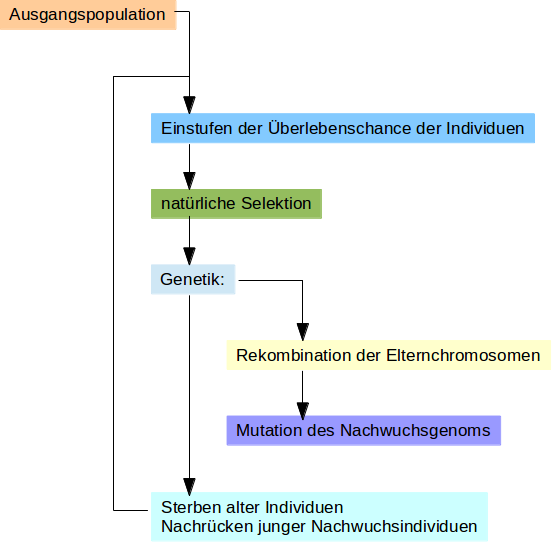
\includegraphics[width=\textwidth]{GenAlg-Diagramm.png}
        \captionsource{\tiny Evolutionäre Algorithmen zur Parametereinstellung
          in elektrophysiologischen Neuronenmodellen, Anne Kloskowski, 2013}
    \end{column}
  \end{columns}
\end{frame}


\subsection{GUI}

\begin{frame}
  \frametitle{GUI}
  \center
  \LARGE
  Anwendungsbeispiel
\end{frame}

\subsection{Ergebnisse}

\begin{frame}
  \frametitle{Durchführung}
  \begin{itemize}
  \item 44 Simulationen
  \item eine Baseline je Neuronklasse
    \scriptsize
    \begin{tabular}[H]{ll}
      Parameter & Werte \\\hline
      Populationsgröße & 50, 125, 200 \\ \arrayrulecolor{light-gray}\hline
      Tournament Selection, Tournamentgröße & 5, 15 \\
      Fitness Proportionate Selection & \\
      Truncation Selection  & \\ \hline
      Mutationsstärke & 0.08333, 0.15, 0.25 \\ \hline
      Random Replacement, elites & 0, 5, 10 \\
      Truncation Replacement & \\
    \end{tabular}
  \end{itemize}
\end{frame}

\begin{frame}
  \frametitle{Durchführung}
  Baseline-Einstellungen
  \begin{itemize}
    \item zufällige Startpopulation in den Grenzen
    \item Tournament Selection (Tournamentgröße 5)
    \item 1-Point-Crossover (Crossover Rate 0.25)
    \item Nonuniform Mutation (Mutationsstärke 0.15)
    \item Truncation Replacement
    \item Populationsgröße 125
    \item 60 Generationen
  \end{itemize}
  \only<2->{
    \center
    Idee: Veränderung der Parameter, Auswertung der Ergebnisse
  }
\end{frame}


% RS: mut-strength(alle)
% IB: popsize(alle)
% FS: alle selections, 4 Stück
% CH: alle replacer, 4 Stück
\begin{frame}
  \frametitle{Regular Spiking}
  \begin{figure}
    \centering
    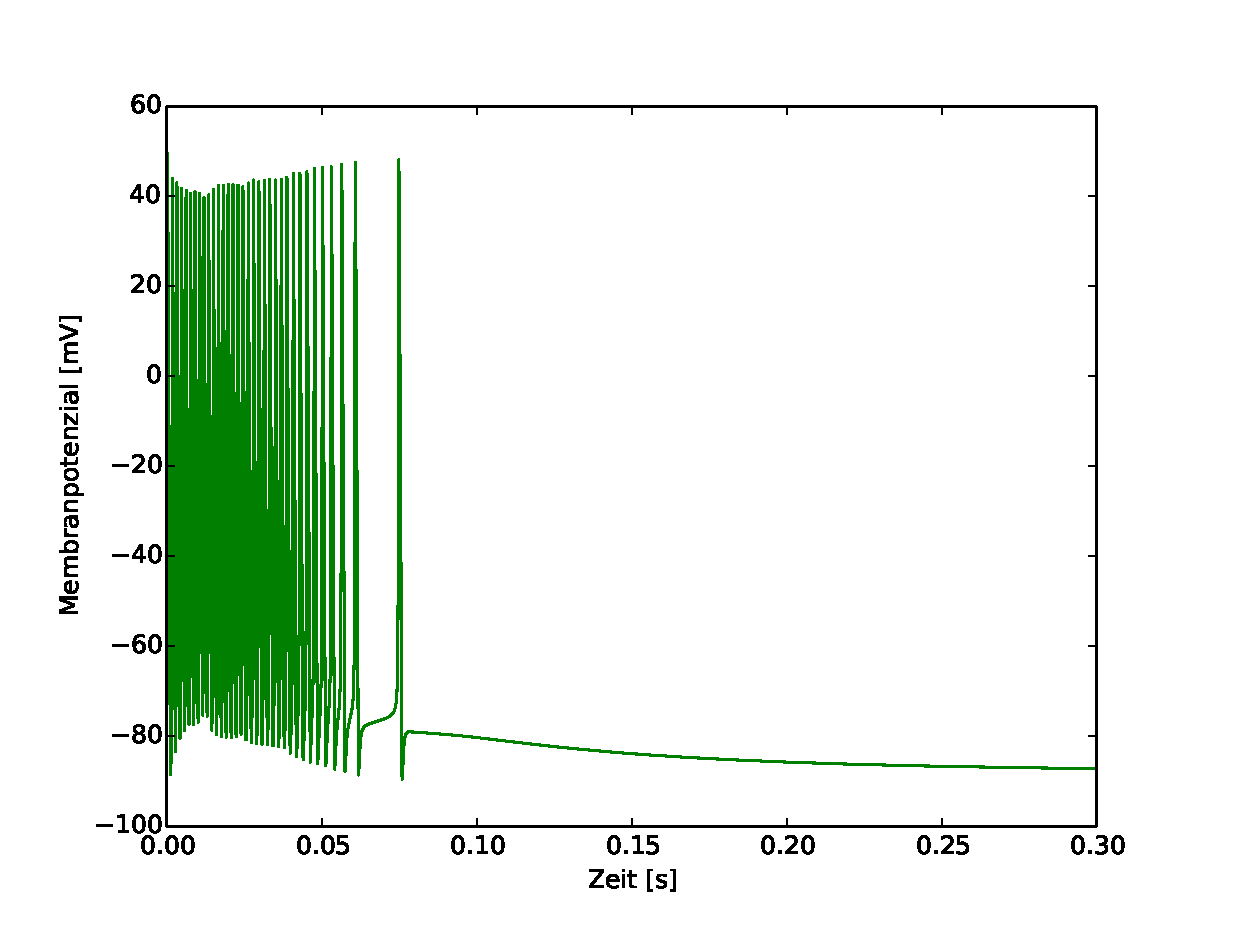
\includegraphics[viewport=19 10 532 394,width=0.35\linewidth]{genetic/rs-base.eps}
    \caption*{\scriptsize{Mutationsstärke 15 \%} \tiny{Fitness: -103}}
    \begin{subfigure}{.5\textwidth}
      \centering
      \includegraphics*[viewport=19 10 532 394,width=0.7\linewidth]{genetic/rs-mut008333.eps}
      \caption*{\scriptsize{Mutationsstärke 8.333 \%} \tiny{Fitness: -150}}
    \end{subfigure}%
    \begin{subfigure}{.5\textwidth}
      \centering
      \includegraphics*[viewport=19 10 532 394,width=0.7\linewidth]{genetic/rs-mut025.eps}
      \caption*{\scriptsize{Mutationsstärke 25 \%} \tiny{Fitness: -107}}
    \end{subfigure}
  \end{figure}
\end{frame}

\begin{frame}
  \frametitle{Intrinsic Bursting}
  \begin{figure}
    \centering
    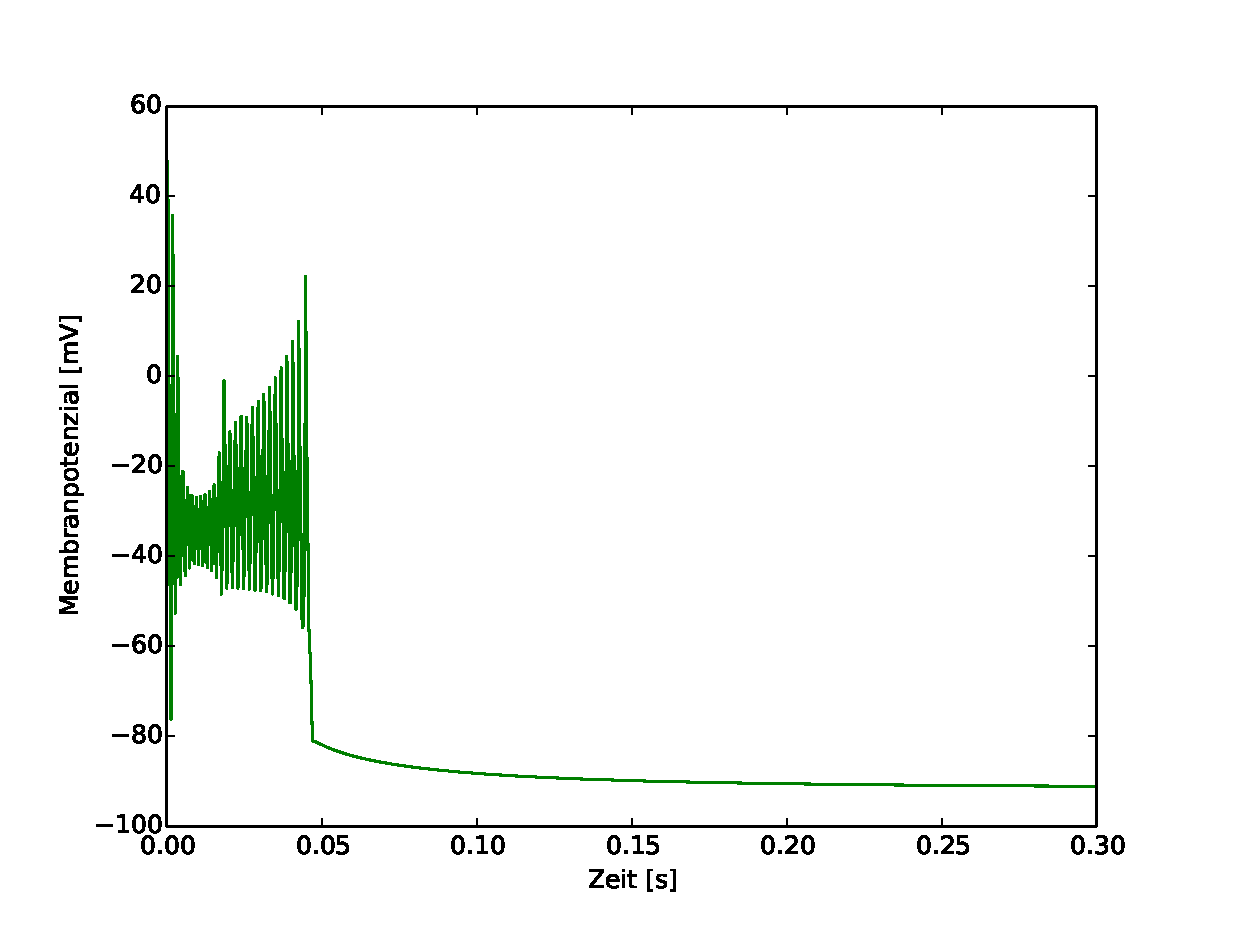
\includegraphics[viewport=19 10 532 394,width=0.35\linewidth]{genetic/ib-pop200.eps}
    \caption*{\scriptsize{Populationsgröße 200} \tiny{Fitness: -358}}
    \begin{subfigure}{.5\textwidth}
      \centering
      \includegraphics*[viewport=19 10 532 394,width=0.7\linewidth]{genetic/ib-pop50.eps}
      \caption*{\scriptsize{Populationsgröße 50} \tiny{Fitness: -588}}
    \end{subfigure}%
    \begin{subfigure}{.5\textwidth}
      \centering
      \includegraphics*[viewport=19 10 532 394,width=0.7\linewidth]{genetic/ib-base.eps}
      \caption*{\scriptsize{Populationsgröße 125} \tiny{Fitness: -531}}
    \end{subfigure}
  \end{figure}
\end{frame}

\begin{frame}
  \frametitle{Fast Spiking}
  \begin{figure}
    \centering
    \begin{subfigure}{.5\textwidth}
      \centering
      \includegraphics*[viewport=19 10 532 394,width=0.7\linewidth]{genetic/fs-base.eps}
      \caption*{\scriptsize{Tournament Selection (TS 5)} \tiny{Fitness: -1354}}
    \end{subfigure}%
    \begin{subfigure}{.5\textwidth}
      \centering
      \includegraphics*[viewport=19 10 532 394,width=0.7\linewidth]{genetic/fs-tsize15.eps}
      \caption*{\scriptsize{Tournament Selection (TS 15)} \tiny{Fitness: -1364}}
    \end{subfigure}
  \end{figure}
  \begin{figure}
    \centering
    \begin{subfigure}{.5\textwidth}
      \centering
      \includegraphics*[viewport=19 10 532 394,width=0.7\linewidth]{genetic/fs-trunc-sel.eps}
      \caption*{\scriptsize{Truncation Selection} \tiny{Fitness: -1374}}
    \end{subfigure}%
    \begin{subfigure}{.5\textwidth}
      \centering
      \includegraphics*[viewport=19 10 532 394,width=0.7\linewidth]{genetic/fs-fitn-prop.eps}
      \caption*{\scriptsize{Fitness-Proportionate Selection} \tiny{Fitness: -1361}}
    \end{subfigure}
  \end{figure}
\end{frame}

\begin{frame}
  \frametitle{Chattering}
  \begin{figure}
    \centering
    \begin{subfigure}{.5\textwidth}
      \centering
      \includegraphics*[viewport=19 10 532 394,width=0.7\linewidth]{genetic/ch-base.eps}
      \caption*{\scriptsize{Truncation Replacement} \tiny{Fitness: -857}}
    \end{subfigure}%
    \begin{subfigure}{.5\textwidth}
      \centering
      \includegraphics*[viewport=19 10 532 394,width=0.7\linewidth]{genetic/ch-rand-repl00.eps}
      \caption*{\scriptsize{Random Replacement (0 El.)} \tiny{Fitness: -2757}}
    \end{subfigure}
  \end{figure}
  \begin{figure}
    \centering
    \begin{subfigure}{.5\textwidth}
      \centering
      \includegraphics*[viewport=19 10 532 394,width=0.7\linewidth]{genetic/ch-rand-repl05.eps}
      \caption*{\scriptsize{Random Replacement (5 El.)} \tiny{Fitness: -873}}
    \end{subfigure}%
    \begin{subfigure}{.5\textwidth}
      \centering
      \includegraphics*[viewport=19 10 532 394,width=0.7\linewidth]{genetic/ch-rand-repl10.eps}
      \caption*{\scriptsize{Random Replacement (10 El.)} \tiny{Fitness: -849}}
    \end{subfigure}
  \end{figure}
\end{frame}

\begin{frame}
  Fazit
  \begin{itemize}
    \item{Populationsgröße nicht ausschlaggebend}
    \item{Fitness-Werte kein gutes Maß}
  \end{itemize}
  
  \only<2->{
    \ \\
    \ \\
    Aussicht
    \begin{itemize}
      \item Anpassung der Fitnessfunktion
      \item mehrfache Ausführung der Läufe
      \item Kombination von zielführenden Parametern
    \end{itemize}
  }
\end{frame}